\section{Linear TM Overlay}

\subsection{Architecture Description}
We propose to build a linear array of FUs as a time-multiplexed (TM) overlay~\cite{li2018time} where each FU can be time multiplexed among operations present in a single scheduling stage of a directed acyclic graph (DAG). 
The 32-bit linear TM overlay is comprised of a quasi-streaming data interface made up of two FIFO channels implemented using Block RAMs, which transmit the data through daisy-chained fully pipelined time-multiplexed FUs, as shown in Figure~\ref{overlay}. 

\begin{figure}
    \centering
	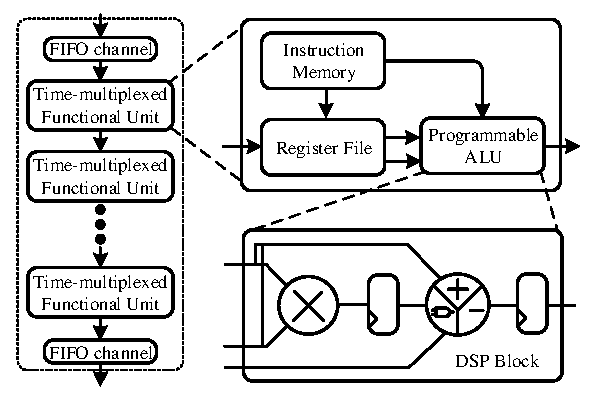
\includegraphics[width=\columnwidth]{Figures/overlay.pdf}
	\caption{A linear TM overlay.}
	\label{overlay}
\end{figure}

\subsection{FU Microarchitecture}
The proposed FU is a simplification of the iDEA soft processor~\cite{cheah2012idea}, which is a DSP based fully functioning CPU optimized to achieve maximum speed on a Xilinx FPGA. 
However, our FU does not require this full functionality as data is moved through the overlay in a quasi-streaming fashion. 
As such, there is no need for large instruction or data memory blocks based on BRAM primitives, as is seen in other CGRA-like overlays~\cite{liu2013soft,paul2012remorph}. 
%Adding the initial requirement
Instead, a smaller instruction memory (IM) can be used. 
Examining the typical overlay benchmark examples from the literature~\cite{binipolynomial, gopalakrishnan2007finding}, it was determined that a depth 32 IM could be used as the identified benchmarks could all fit within this constraint. 
As such, a 32$\times$32-bit IM can be implemented using LUTRAM based RAM32M primitives, resulting in a 5-bit instruction counter (IC) and a 5-bit program counter (PC). 
Similarly, a 32$\times$32-bit rotating register file (RRF) is instantiated using RAM32M primitives. 
The ALU of an FU is based on a DSP block with three stage pipelining for maximum speed. 
Initially, a tag is required for each instruction to match with its corresponding FU as configuration data (e.g. instructions) is streamed through the array from FU to FU. 
It is customized as an 8-bit tag combined with the 32-bit instructions, which can support up to 256 FUs. 
This dedicated design results in some simplifications to the FU architecture, with a reduction in the number of pipeline stages compared to iDEA~\cite{cheah2012idea}.
The FU has an execution pipeline with 7 stages in total, with a latency of 1-clock cycle per stage. These are divided as follows: 2 stages for instruction fetch, 2 stages for operand indexing, and 3 stages for instruction execute.
As the FU operates as a streaming processing element and the feedback data is written back to the RRF, data memory is not required in the FU. 


\subsubsection{Instruction Memory}
The instruction memory (IM) is used to store the list of instructions that are performed in the DAG scheduling stage. 
To enable the simple and efficient configuration of the full overlay, the FU instruction ports are connected in series (in a daisy-chained manner). Then, at initialization, or upon a hardware context switch, the FU context is clocked to the FU instruction port from a separate 40-bit wide context memory. This 40-bit data word consists of a 32-bit wide instruction (the kernel$\mbox{'}$s context) and an 8-bit tag (used to match an instruction with its corresponding FU). The context memory is implemented externally using BRAMs. 
A 5-bit instruction counter (IC) is used to keep track of the specific instructions written to each FU. 
%There are two types of instruction: arithmetic and data bypass (used to forward data to the next stage).
There are just two types of instructions. The first type are the arithmetic instructions used for computing purposes while the second type are data bypass instructions needed to feed input data to the next scheduling stage. 

The FU microarchitecture uses a 32 entry IM implemented using RAM32M primitives, which enables an efficient LUT-based IM implementation.  The RAM32M primitive can be configured as a 32 deep 2-bit wide quad port (3-read, 1-read/write), a 32 deep 4-bit wide dual port (1-read, 1-read/write) or a 32 deep 8-bit wide single port (1-read/write) memory.
As IM writes only occur infrequently (just once at context initialization), we adopt a single port configuration where the read and write addresses are multiplexed. This configuration uses only four RAM32M primitives for a 32$\times$32 IM. 
An extra pipeline stage is added to the output of the RAM32M primitive to ensure that it operates at close to its maximum frequency. 
The \textit{inst\_fetch} signal (at the output of the IM block) represents the instruction which has been read from the IM block, and appears 2 clock cycles after the program counter (PC) initiates the instruction fetch, as shown in Figure~\ref{fu_wb}. 
A description of the 32-bit internal instruction format, using \textit{ADD R3, R5 (WB)} operation as an example, is shown in Table~\ref{instruction}. 
From this table, it can be seen that a 32-bit instruction has four sections, the 18-bit ALU control, the 2-bit input map multiplexing, two 5-bit source operand addresses, with the remaining 2-bit reserved for future use. 
At the end of the FU context write cycle, each FU contains the instructions that it needs to execute (in the IM) and the number of instructions that it needs to execute (in the IC register). 

\begin{table*}
	\renewcommand{\arraystretch}{1.2}
	\caption{Instruction format.}
	\label{instruction}
	\scriptsize
	\centering
	\resizebox{\textwidth}{!}{	
		\begin{tabular}{|c|c|c|c|c|c|c|c|c|c|c|c|c|c|}
			\hline
			        FU part          &                         \multicolumn{8}{c|}{ALU Control}                         & \multicolumn{2}{c|}{Input Map Control} & \multicolumn{2}{c|}{RF Control} & Reserved \\ \hline
			        Signals          & \textit{NDF} & \textit{WB} & alumode & inmode  & opmode  & cea2 & ceb2 & usemult & split &             immop              & src-1  &         src-2          &  \\ \hline
			      No. of bits        &      1       &      1      &    4    &    2    &    7    &  1   &  1   &    1    &   1   &               1                &   5    &           5            &    2     \\ \hline
			       Locations         &     [30]     &    [29]     & [28:25] & [24:23] & [22:16] &  15  &  14  &   13    &  12   &               11               & [10:6] &         [5:1]          & [31][0]  \\ \hline
			ADD R3, R5 (\textit{WB}) &      0       &      1      &  0000   &   00    & 0110011 &  1   &  1   &    0    &   1   &               0                & 00011  &         00101          &   0 0    \\ \hline
		\end{tabular}}
	\end{table*}
	
\subsubsection{Rotating Register File}
%On the availability of data at the input FIFO channel for processing, instruction memory waits until data gets buffered in the register file. 
The rotating register file (RRF) is used for 32-bit temporary data storage, including the data from the input FIFO (or the previous FU stage) and the feedback data from the FU output. 
When valid data is available from the input FIFO (or previous stage), the data counter (DC) controls the data transfer to the RRF using simulated load instructions. 
Data transfer is initiated by the \textit{valid\_in} signal going high, indicating that data is being streamed into the FU. 
For each transfer, the DC is incremented resulting in data being written into the RRF in sequential locations. 
When the data transfer is complete and all data is available in the register file the \textit{valid\_in} signal goes low. 
The control logic (control generator) then asserts a \textit{control} signal to indicate to the IM that it should start sending operand addresses to the RRF and configuration data to the DSP block, with the specific instruction to be executed determined by the PC. 
To efficiently support the overlap of data written into the RF with the execution of subsequent instructions, we developed an RRF which is different from the normal register file (RF) in two aspects. 
First, the DC will never be reset so that the input data is written into successive locations of the RRF in a rotating way, one data packet after another. 
Second, an offset counter (shown as the circuitry inside the middle dashed box) is added to update the read address index, eliminating the offset deviation caused by this rotating mode. 
Therefore the 32 entry RRF requires 16 RAM32M primitives configured as a 2-read and 1-write port memory (32-deep by 2-bit wide). 
Similar to the IM, there is an extra pipeline register at the output of the RAM32M-based RRF to ensure maximum operating frequency. 
Thus, it takes 2 cycles to source the operands from the RRF for a specific instruction (\textit{inst\_fetch}). 
Hence, the \textit{inst\_exec} signal to the DSP block and the input map logic requires two additional register stages to ensure synchronization, as shown in Figure~\ref{fu_wb}. 
After executing all the instructions in the FU IM, including any data forwarding to the next stage (or the output FIFO), the program counter resets. This then flushes the DSP block's internal pipeline and allows the same sequence of instructions to be executed again. This mechanism reduces the size required for the IM as there is no need to store a large number of instructions for each cycle, resulting in a smaller IM and RRF design. 

\subsubsection{Computing Unit}
The block responsible for computational operations is the computing unit, which consists of a DSP block, a 32-bit register at the C input port for pipeline balancing, and an 19-bit register for the DSP configuration. 
The DSP block has a pre-adder, a multiplier, an ALU, four input ports and one output port. 
It supports various operations such as MULTIPLY, ADD, SUB, bitwise logical operations, etc., which are determined by a set of dynamic control inputs connected to the configuration registers. 
An instruction decoder is not required as there are sufficient instruction bits to specify the read addresses of the RRF and the modes of operation of the DSP block directly. This avoids unnecessary pipeline stages while achieving a relatively high frequency. 

\begin{figure*}
	\centering
	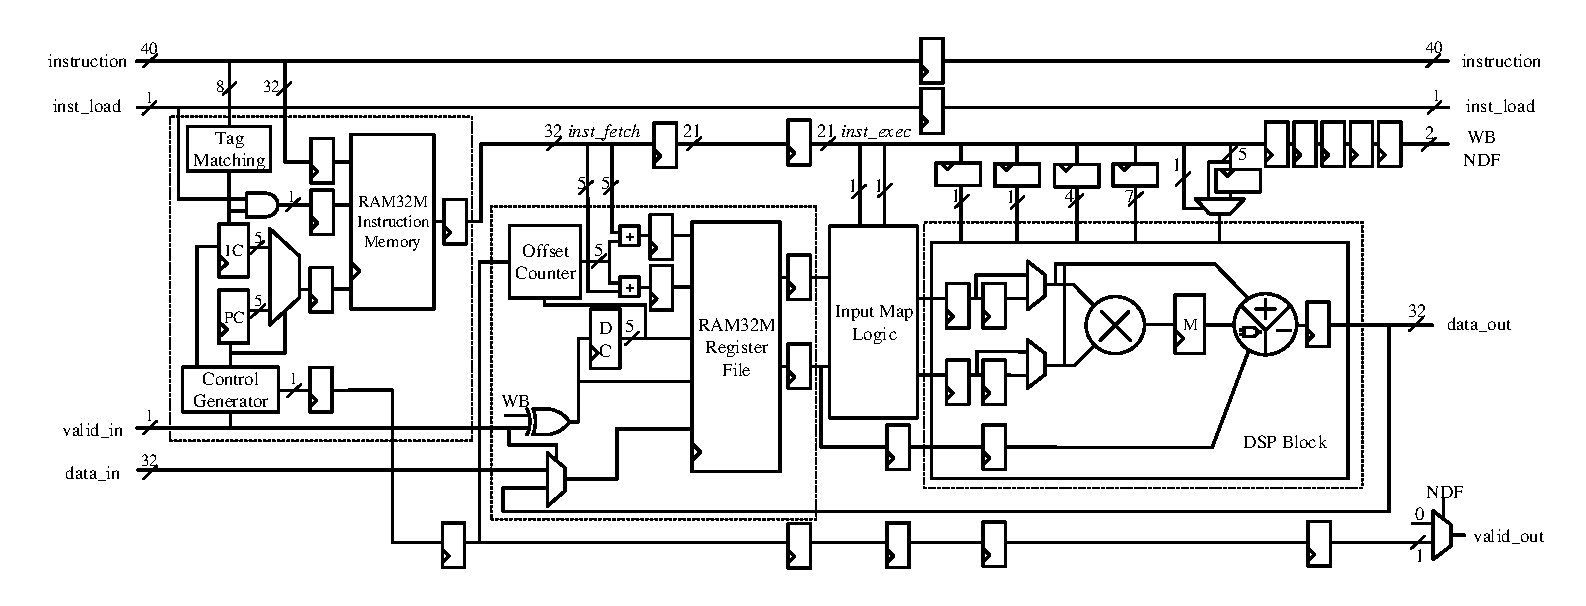
\includegraphics[width=\linewidth]{Figures/FU_WB.pdf}
	\caption{FU microarchitecture.}
	\label{fu_wb}
\end{figure*}

\subsection{Overlay Control and Functionality}
%\textbf{(a) Back-pressure Control}
A back-pressure control circuit is built around the input FIFO channel to manage the functionality of the proposed overlay, as shown in Figure~\ref{back_pressure}. 
There are three control signals which indicate the duration for instruction load, overlay setup and data write respectively, referred to as \textit{inst\_load}, \textit{reg\_wren}, and \textit{data\_wren}. 
Initially, FU instructions are read from the memory and streamed through the daisy-chained FUs. During instruction load (when the \textit{inst\_load} is high), both the write enable port of the FIFO and the valid signal (\textit{valid\_out}) for data output are disabled. 
After instruction load, two integers are written to the back-pressure control circuit. The first represents the number of data words to be input to the first FU for a specific compute kernel while the other is equal to the II minus one (II-1) and determines the interval between data loads. These values are written into the controller when the \textit{reg\_wren} signal is active (high). 
The process of instruction load and overlay setup represent the initialization of the overlay.
	
\begin{figure*}
	\centering
	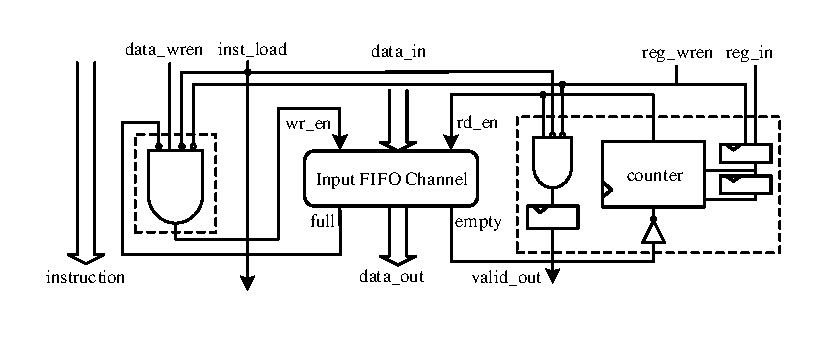
\includegraphics{Figures/control.pdf}
	\caption{Back-pressure control circuit.}
	\label{back_pressure}
\end{figure*}
	
The dashed box on the left hand side of Figure~\ref{back_pressure} acts as the control module for the write enable port of the FIFO, while the other dashed box on the right hand side contains the logic to control the read enable port of the FIFO. 
The write enable signal (\textit{wr\_en}) is determined as shown in the truth table of Table~\ref{truth_table}. 
Data is written into the FIFO when \textit{wr\_en} is high.
The read enable signal (\textit{rd\_en}) for the FIFO is generated from a counter which determines the number of cycles needed to load input data to the FU. 
The counter starts counting from 0 when the \textit{empty} signal goes low (indicating that data is available in the FIFO). The counter counts up until the count value equals II-1, at which point it rolls over back to zero.   
The \textit{rd\_en} signal is valid only while the counter is less than the initial number loaded into the back-pressure circuit, limiting the amount of data to be loaded into the first FU.
Once the counter value is greater than or equal to the data load number (in the back-pressure circuit), the \textit{rd\_en} signal is forced low and the input data is buffered in the FIFO.
	
\begin{table}
%	\renewcommand{\arraystretch}{1.2}
	\centering
	\caption{Truth table of the \textit{wr\_en} signal.}
	\label{truth_table}
	%\begin{displaymath}
	%\begin{array}{|c c c c |c|}
	\begin{tabular}{c c c c |c}
		\hline
		\textit{inst\_load} & \textit{reg\_wren} & \textit{data\_wren} & \textit{full} & \textit{wr\_en} \\ \hline
		         0          & 0                  & 0                   & 0             & 0               \\
		         0          & 0                  & 0                   & 1             & 0               \\
		         0          & 0                  & 1                   & 0             & 1               \\
		         0          & 0                  & 1                   & 1             & 0               \\
		         0          & 1                  & 0                   & 0             & 0               \\
		         0          & 1                  & 0                   & 1             & 0               \\
		         0          & 1                  & 1                   & 0             & 0               \\
		         0          & 1                  & 1                   & 1             & 0               \\
		         1          & 0                  & 0                   & 0             & 0               \\
		         1          & 0                  & 0                   & 1             & 0               \\
		         1          & 0                  & 1                   & 0             & 0               \\
		         1          & 0                  & 1                   & 1             & 0               \\
		         1          & 1                  & 0                   & 0             & 0               \\
		         1          & 1                  & 0                   & 1             & 0               \\
		         1          & 1                  & 1                   & 0             & 0               \\
		         1          & 1                  & 1                   & 1             & 0               \\ \hline
	\end{tabular}
	%\end{array}
	%\end{displaymath}
\end{table}
	
%\textbf{(b) Overlay Functionality}
The working mechanism of the proposed overlay is shown in Figure~\ref{flow_chart}, illustrated using `gradient' benchmark from the medical imaging domain~\cite{cong2014fully}. 
As can be seen from Figure~\ref{flow_chart}, the initialization of the overlay for the `gradient' benchmark takes 22 clock cycles in total, consisting of 20 cycles for instruction load and 2 cycles for overlay back-pressure configuration. 
Then, input data is fed into the FIFO in a streaming fashion with an II of 6. 
The latency (44 cycles) is obtained by calculating the interval between the input of the first FU and the output of the last FU. 

\begin{figure*}
	\centering
	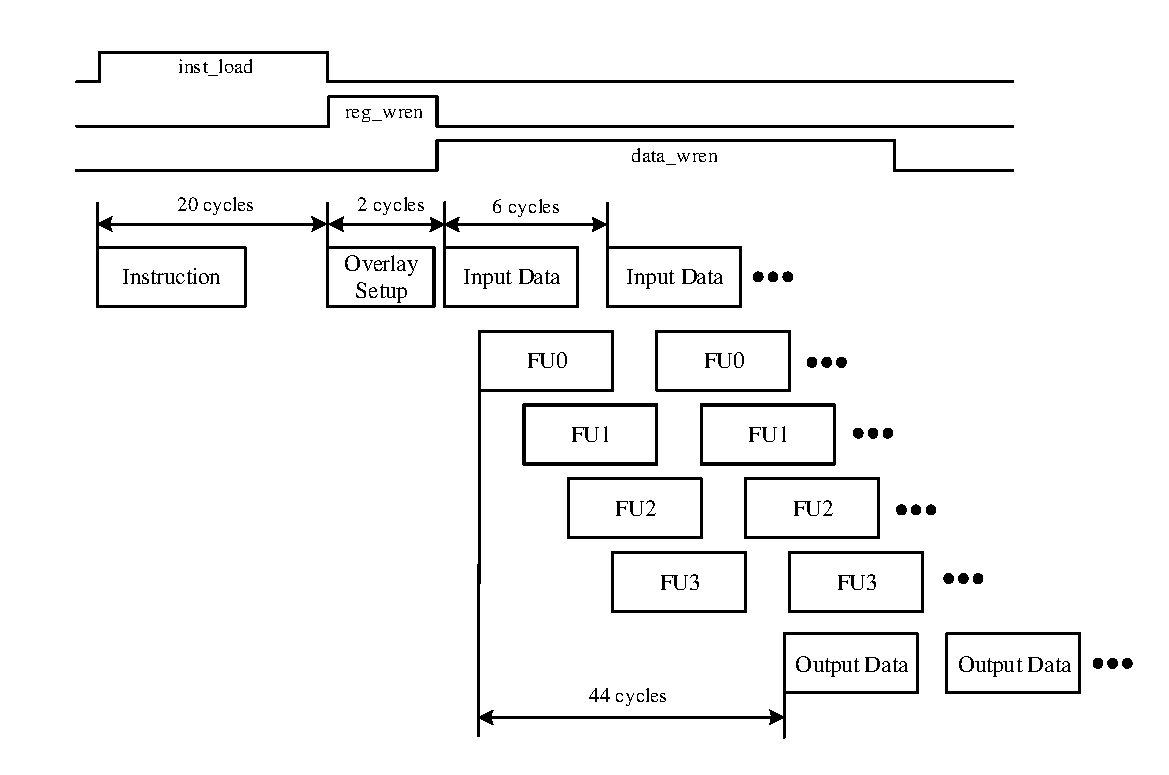
\includegraphics[width=0.9\linewidth]{Figures/flow_chart.pdf}
	\caption{Flow chart of overlay functionality.}
	\label{flow_chart}
\end{figure*}
